\documentclass[12pt]{article}

\usepackage{fancyhdr}
\usepackage{geometry}
\usepackage{ucs}
\usepackage[utf8x]{inputenc}
\usepackage[T1]{fontenc}
\usepackage[ngerman]{babel}
\usepackage{amsmath,amssymb,amstext}
\usepackage{hyperref}
\usepackage{cancel}
\usepackage{dsfont}
\usepackage{physics}
\usepackage{lmodern}
\usepackage{enumerate}
\usepackage{enumitem}
\usepackage{graphicx}
\usepackage{listings, color}
\usepackage[labelfont=bf]{caption}
\usepackage{titling}

\lstset{basicstyle=\scriptsize} %Quellcode mit Umlauten und ganz klein
\lstset{literate=
  {Ö}{{\"O}}1
  {Ä}{{\"A}}1
  {Ü}{{\"U}}1
  {ß}{{\ss}}2
  {ü}{{\"u}}1
  {ä}{{\"a}}1
  {ö}{{\"o}}1
}


%Geometrie----------------------------------------------------------------------------------------------------------

\geometry{a4paper, top=25mm, left=15mm, right=15mm, bottom=25mm,headsep=10mm, footskip=10mm}
\pagestyle{fancy}
\setlength{\parindent}{0pt} %Zeileneinrückung

\fancyhf{} %Setzt voreingestellte Kopf-und Fußzeilen-Eigenschaften zurück

\lhead{\nouppercase{\leftmark}}
\chead{}
\rhead{\thepage}

\lfoot{}
\cfoot{}
\rfoot{}

\title{\vspace{0cm}{\Huge Fortgeschrittenen-Praktikum I:\\ \vspace{1cm} Kernspinresonanz}}
\author{Saskia Bondza\\Simon Stephan}
\date{durchgeführt am 15.09.2016}

\pretitle{%
  \begin{center}
  \LARGE
  
\includegraphics[width=6cm,]{figures/siegel}\\[\bigskipamount]
}
\posttitle{\end{center}}

%neue Commands----------------------------------------------------------------------------------------------------------
\newcommand{\nab}{\vec{\nabla}} %direkter Befehl mit Vektorpfeil
\newcommand{\gra}[3][0.7]{
	\begin{minipage}[h!]{\textwidth}
		\centering
		\includegraphics[width=#1\textwidth]{figures/#2.png}
		\captionof{figure}{#3}
	\end{minipage}
	\vskip 30 pt
}
\newcommand{\graTwo}[4][0.5]{
	\begin{minipage}[h!]{\textwidth}
		\centering
		\includegraphics[width=#1\textwidth]{figures/#2.png}
		\includegraphics[width=#1\textwidth]{figures/#3.png}
		\captionof{figure}{#4}
	\end{minipage}
	\vskip 30 pt
}
\newcommand{\code}[1]{\texttt{#1}}


%Titel,Inhalt----------------------------------------------------------------------------------------------------------

\begin{document}
\pagenumbering{gobble} %verstecke Seitenzahl
\maketitle
\newpage

\thispagestyle{empty}
\tableofcontents
\newpage

%Schreiben----------------------------------------------------------------------------------------------------------
\pagenumbering{arabic} %verstecke Seitenzahl
\section{Einleitung}

In diesem Versuch untersuchen wir Kernspinresonanz. Dieser Effekt beruht auf dem Zeeman-Effekt und beschreibt das Umklappen von Kernspins in einem Magnetfeld unter Absorption oder Emission von Photonen. Wir benutzen die Kernspinresonanz um das gyromagnetische Verhältnis des Protons einmal in Wasserstoff und einmal in Glykol zu bestimmen. Anschließend messen wir das kernmagnetische Moment von $^{19}$F und die Protonenresonanzfrequenz von Wasserstoff. Außerdem untersuchen wir das in diesem Versuch benutzte magnetische Feld mit einer Hall-Sonde, um dessen Homogenität zu bestätigen.


\newpage
\section{Theoretische Grundlagen}
In diesem Kapitel haben wir uns weitgehend an \cite{anleitung} orientiert.
\subsection{Spin und Kernspin}\label{CURVEFEVER3SUCKS}
Eine wichtige Eigenschaft quantenmechanischer Elementarteilchen ist ihr Spin. Dieser beschreibt, halbklassisch gesehen, die Rotation eines Teilchens um den eigenen Schwerpunkt. Der Spin besitzt eine Quantenzahl $S=0,\frac12,1,\frac32,...$. Die möglichen Beträge sind $|\vec S|=\hbar\sqrt{S(S+1)}$.\\

Nicht nur Elementarteilchen sondern auch Atomkerne besitzen einen Spin. Dieser sogenannte Kernspin wird wie folgt definiert: $|\vec I|=\hbar\sqrt{I(I+1)}$. Die Projektion des Kernspins auf die Quantisierungsachse $z$ ist $I_z=m_I\hbar$ mit $-I\leq m_I\leq +I$, womit es $2I+1$ Einstellmöglichkeiten für $I_z$ gibt.\\

Der Spin eines Kerns setzt sich aus den Spins seiner Nukleonen zusammen. Aufgrund des Pauli-Prinzips wird jedes Orbital im Grundzustand durch zwei Neutronen oder zwei Protonen entgegengesetzten Spins besetzt. Bei gg-Kernen (jeweils gerade Anzahl an Neutronen und Protonen) sind die Orbitale gefüllt und es ergibt sich ein Gesamtspin $I=0$. Für uu-Kerne (jeweils ungerade Anzahl an Neutronen und Protonen) erhält man einen ganzzahligen Kernspin. Für ug- und gu-Kerne erhält man also einen halbzahligen Kernspin.\\

Die in diesem Versuch betrachteten Kerne, das Proton und der $^{19}$F-Kern mit 9 Protonen und 10 Neutronen haben also einen Spin $I=\frac12$. Für diese gibt es nun also genau zwei Einstellmöglichkeiten: $m_I=\frac12$ und $m_I=-\frac12$, also parallelen und antiparallelen Spin.

\subsection{Magnetisches Moment}
Der Spin eines quantenmechanischen Teilchens erzeugt immer ein magnetisches Dipolmoment $\vec\mu$, das kernmagnetische Moment. Es gilt $\vec\mu=\gamma\vec I$, wobei $\gamma=\frac{g_I\mu_k}{\hbar}$ das gyromagnetische Verhältnis ist. $g_I$ ist der sogenannte Kern-g-Faktor, welcher auch in diesem Versuch bestimmt werden soll. Dieser Faktor ist charakteristisch für den jeweiligen Kern. $\mu_k$ ist das Kernmagnetron mit $\mu_k=\frac{e\hbar}{2m_p}$.

\subsection{Zeeman-Effekt und Kernspinresonanz}
Ein Kern mit einem kernmagnetischen Moment hat in einem magnetischen Feld in z-Richtung die Energie $E==-\vec\mu\cdot\vec B=-g_I\mu_km_IB$. Die Energiezustände des Kerns sind also aufgespalten nach ihrem Kernspin. Dieser Effekt ist der Zeeman-Effekt. Der Abstand zweier benachbarter Zustände ist nun $\Delta E=g_I\mu_k B$.\\

Übergänge zwischen diesen beiden Zuständen können durch spontane oder induzierte Emission oder Absorption von Photonen auftreten. Die Energie, die dazu benötigt wird oder frei wird, beträgt genau $\Delta E$. Photonen eines Strahlungsfeldes, welches diese Übergänge hervorrufen soll, müssen also die Frequenz $\nu=\frac{\Delta E}{h}=\frac{g_i\mu_kB}{h}=\frac{\gamma B}{2\pi}$ haben.\\

Wenn ein Kern im energetisch niedrigeren Zustand nun ein Photon absorbiert und in einen energetisch höheren Zustand wechselt, also der Spin umklappt, dann gibt das Photon seine Energie an den Kern ab, wodurch das Strahlungsfeld an Intensität verliert. Umgekehrt kann der Kern vom energetisch höheren in den energetisch niedrigeren Zustand wechseln und dabei die Energie $\Delta E$ an ein Photon abgeben. Dadurch wird die Intensität des Strahlungsfeldes wiederum erhöht.\\

Die Energieniveaus des Kerns gehorchen im thermischen Gleichgewicht einer Boltzmann-Verteilung. Also beträgt das Verhältnis der Besetzungszahlen des energetisch höheren zum energetisch niedrigeren Zustandes $\frac{n_{\text{hoch}}}{n_{\text{tief}}}=\exp\left(-\frac{\Delta E}{kT}\right)$ mit der Boltzmann-Konstante $k$ und der Temperatur $T$. Insgesamt bilden sich also immer mehr Teilchen im energetisch niedrigeren als im energetisch höheren Zustand. Deshalb verliert das Strahlungsfeld Energie, welches sich im Versuch als Dämpfung eines elektromagnetischen Schwingkreises zeigt.

\subsection{Relaxation}
Da mehr Kerne vom energetisch tieferen in den höheren Zustand gehen als umgekehrt, müsste es nun bald genauso viele Kerne im höheren wie im tieferen Zustand geben. Dann würde sich die Zahl der Absorption mit der Zahl der Emissionen decken und es gäbe keine messbare Dämpfung des Schwingkreises mehr.\\

Es gibt allerdings Effekte, die Relaxationsprozesse, welche den Besetzungsunterschied aufrecht erhalten. Dies ist zum Einen die Spin-Gitter-Relaxation, bei welcher die Kerne im energetisch höheren Zustand ihre Energie strahlungslos als thermische Energie an die Molekülstruktur abgeben. Zum Anderen ist dies die Spin-Spin-Relaxation. Dieser Prozess beschreibt das Magnetfeld, welches durch den Spin eines Kerns am Ort eines anderen Kerns erzeugt wird. Das gesamte Magnetfeld am Ort des anderen Kerns ist nun also etwas stärker oder schwächer als das äußere Magnetfeld. Dadurch verschiebt sich die Resonanzfrequenz des Kerns, was zu einer Verbreiterung der Absorptionslinie führt.

\subsection{Hallsonde}

Auf bewegte Elektronen in einem Magnetfeld wirkt die Lorentzkraft. Diese lenkt die Elektronen senkrecht zu ihrer Bewegungsrichtung aus. Dadurch werden die Elektronen in einem stromdurchflossenen Leiter an den Rand dieses Leiters bewegt. Also bildet sich ein elektrisches Feld zwischen den beiden Seiten des Leiters. Die daraus folgende elektrische Kraft bildet ein Kräftegleichgewicht mit der Lorentzkraft. Sie Spannung zwischen den beiden Seiten des Leiters lässt sich nun von außen mit einem Voltmeter messen, dies ist die sogenannte Hallspannung (siehe Abbildung \ref{hallsonde}). Mit $F_{\text{el}}=q\cdot E=q\cdot\frac Ud$ und $F_{\text{Lorentz}}=q\cdot v\cdot B$ gilt nun $U=d\cdot v\cdot B$, womit sich durch Messung der Spannung das Magnetfeld bestimmen lässt. Das hier beschriebene Gerät zur Messung des Magnetfelds nennt sich Hallsonde nach dem Entdecker Edwin Hall \cite{bibhall}.

\gra[0.5]{halleffekt}{Funktionsweise einer Hallsonde \label{hallsonde}\cite{bibhall}}

\subsection{Messung der Kernspinresonanzfrequenz}\label{messung1}
\gra[0.5]{messprinzip1}{Absorptionsminima am Oszilloskop mit äquidistantem Abstand \label{messprinzip1}\cite{anleitung}}

Zum Messen der Kernspinresonanzfrequenz stellen wir das Strahlungsfeld auf eine vermutete Resonanzfrequenz ein und variieren das Magnetfeld. Die Verluste im Strahlungsfeld bei Überfahren der Resonanz zeigen sich durch Minima in der Absorptionskurve. Um die Resonanzfrequenz nun bestimmen zu können modulieren wir das B-Feld mit einer Sinus-Kurve. Bei exaktem Treffen der Resonanzfrequenz sind die Absorptionsminima äquidistant (siehe Abbildung \ref{messprinzip1}). Die Frequenz wird nun so eingestellt, dass die Absorptionsminima äquidistant sind, um die Resonanzfrequenz zu erhalten.

\subsection{Messung der Kernspinresonanzfrequenz mithilfe des Lock-In-Verfahrens}\label{messung2}
\gra[0.5]{messprinzip2}{Differenziertes Absorptionsbild \label{messprinzip2}\cite{anleitung}}


Bei der in \ref{messung1} beschriebenen Messung kann der Wert nicht sehr genau eingestellt und gemessen werden. Um eine bessere Messung zu erhalten, benutzen wir in einer Messreihe das Lock-In-Verfahren, durch das wir ein differenziertes Signal erhalten. Dazu modulieren wir das Magnetfeld mit einer Sägezahnkurve, auf die ein Sinussignal kleiner Amplitude und hoher Frequenz aufgesetzt wird (siehe Abbildung \ref{messprinzip2}. Das Absorptionssignal wird in einem sogenannten Synchrondetektor mit einem Referenzsignal multipliziert, durch einen Tiefpassfilter integriert und anschließend verstärkt. So werden Störsignale durch Rauschen oder andere Effekte unterdrückt.\\

Aus den unterschiedlichen zeitlichen Abständen $\Delta t$ der Nulldurchgänge des Absorptions- und Sägezahnsignals bei mehreren Frequenzen kann nun durch Interpolation die Resonanzfrequenz berechnet werden.


\newpage
\section{Versuchsaufbau und -Durchführung}

\subsection{Vermessung des Magnetfelds}
\gra[0.5]{aufbau1}{Schaltbild für die Vermesung des Magnetfelds \label{aufbau1}\cite{anleitung}}

Zu Beginn des Versuchs vermessen wir das Magnetfeld und überprüfen dessen Homogenität. Dafür benutzen wir eine Hallsonde, die wir in die Probenöffnung einführen und nun an verschiedenen Höhen das Magnetfeld messen (siehe Abbildung \ref{aufbau1}).

\subsection{Messung der Resonanzfrequenz}

\gra[0.5]{aufbau2}{Schaltbild zur Messung der Resonanzfrequenz \label{aufbau2}\cite{anleitung}}

Zunächst messen wir die Resonanzfrequenzen für das Proton einmal in Wasserstoff und einmal in Glykol und für $^{19}$F einmal rein und einmal in Teflon. Dazu benutzen wir das in \ref{messung1} beschriebene Verfahren und den in Abbildung \ref{aufbau2} beschriebenen Aufbau.

\subsection{Messung der Resonanzfrequenz mithilfe des Lock-In-Verfahrens}

\graTwo[0.49]{aufbau3}{aufbau4}{Schaltbilder zum Lock-In-Verfahren \label{aufbau3}\cite{anleitung}}

Zur Bestimmung der Resonanzfrequenz mithilfe des Lock-In-Verfahrens (siehe \ref{messung2}) stellen wir zunächst die Frequenz grob auf die Resonanzfrequenz ein, um sie später mithilfe des Lock-In-Verfahrens genauer zu untersuchen. Dazu benutzen wir die im linken Teil von Abbildung \ref{aufbau3} beschriebene Schaltung.\\

Anschließend werden die Sägezahnspannung und der Synchrondetektor angeschlossen (siehe Abbildung \ref{aufbau3}) und die Frequenz der Sinusspannung erhöht, während ihre Amplitude verkleinert wird. Nun wird mithilfe des Lock-In-Verfahrens die Resonanzfrequenz des Protons in Wasserstoff genauer vermessen.



\newpage
\section{Auswertung}

\subsection{Homogenität des Magnetfeldes}

Zur Überprüfung der Homogenität des Magnetfeldes tragen wir die gemessenen magnetischen Flussdichten über die zugehörigen Positionen auf. Die Fehlerbalken entsprechen hierbei den Ablesefehlern, also: $s_x = 0.5mm$ und $s_y = 0.5mT$.

\gra{Homo_B}{Überprüfung der Homogenität des Magnetfeldes \label{Homo}}

Aus Abbildung \ref{Homo}  erkennen wir, dass das Magnetfeld in einem Bereich von ca. $10mm$ bis $30mm$ einen konstanten Wert von $407$mT einnimmt, die Homogenität ist damit hinreichend überprüft. Den Betrag der magnetischen Flussdichte bestimmen wir damit im relevanten Bereich (d.h. in unserem Arbeitsbereich) zu $B = 407 \pm 0.5 $mT.
Wir wählen hier den Ablesefehler als Fehler auf den Betrag der magnetischen Flussdichte und keinen fortgepflanzten Mittelwertfehler, da es sich um konstante Werte handelt und durch Bildung eines Mittelwertes keine größere Genauigkeit erreicht wird.  

\subsection{Messmethode 1}

\subsubsection{Resonanzfrequenzen}
\ \\
Wir haben für die verschiedenen Stoffe folgende Resonanzfrequenzen gemessen:

\begin{itemize}
	\item Proton im Wasserstoff: $\nu_{res} = 16.82 \pm 0.01$
	\item Proton in Glycol: $\nu_{res} = 16.85 \pm 0.01$
	\item $^{19}$F:  $\nu_{res} = 15.94 \pm 0.01$
	\item Teflon:  $\nu_{res} = 15.95 \pm 0.01$
\end{itemize}

Die Unsicherheit entspricht dabei nicht der Ablesegenauigkeit sondern ergibt sich aus unserer Abschätzung wie genau eine Resonanzfrequenz einzustellen ist. Diese schätzen wir deutlich größer ein, da zum einen die Anzeige des Geräts schwankt und zum anderen äquidistante Abstände nur bis zu einer gewissen Genauigkeit.
\subsubsection{Proton im Wasserstoff} \label{Rechnung}
\ \\
Wir berechnen zunächst das gyromagnetische Verhältnis aus der Resonanzfrequenz. Aus $\nu=\frac{\gamma B}{2\pi}$ ergibt sich das gyromagnetische Verhältnis zu:

\begin{align*}
\gamma = \frac{2\pi \cdot \nu}{B}
\end{align*}

Der Fehler berechnet sich mit Gauß'scher Fehlerfortpflanzung wie folgt:

\begin{align*}
s_{\gamma} = \sqrt{\left(\frac{s_B}{B}\right)^2+\left(\frac{s_\nu}{\nu}^2 \right)}\cdot \gamma
\end{align*}

Wir erhalten für das Proton in Wasserstoff damit: 

\begin{align*}
\gamma = (2.597\pm 0.004) \cdot 10^8 \frac{1}{Ts}
\end{align*}

außerdem berechnen wir den gyromagnetischen Faktor $g_I$ der sich wie folgt berechnet: 

\begin{align*}
g_I = \frac{\nu \cdot h}{\mu_k \cdot B}
\end{align*}

wobei 
\begin{itemize}
	\item $h =  6.626 \cdot 10^-34 Js$
	\item $\mu_k = 5.05 \cdot 10^-27 J/T$
\end{itemize}

mit dem Fehler:
\begin{align*}
s_{g_I} = \sqrt{\left(\frac{s_B}{B}^2\right)+\left(\frac{s_\nu}{\nu}^2 \right)}\cdot g_I
\end{align*}

Wir erhalten:

\begin{align*}
g_I = 5.422  \pm 0.007
\end{align*}
\subsubsection{Proton in Glykol}
\ \\

Analog zu \ref{Rechnung} berechnen wir hier wieder das gyromagnetische Verhältnis und den gyromagnetischen Faktor aus gemessener Resonanzfrequenz und Magnetfeld. Wir erhalten:

\begin{align*}
\gamma = (2.601\pm 0.004) \cdot 10^8 \frac{1}{Ts}
\end{align*}

\begin{align*}
g_I = 5.432  \pm 0.007
\end{align*}

\subsubsection{$^{19}$Fluor} \label{MEINEXISTEINARSCH}
\ \\

Auch für Fluor berechnen wir zunächst analog zu \ref{Rechnung} das gyromagnetische Verhältnis und den gyromagnetischen Faktor mit folgendem Ergebnis:

\begin{align*}
\gamma = (2.461\pm 0.003) \cdot 10^8 \frac{1}{Ts}
\end{align*}

\begin{align*}
g_I = 5.139  \pm 0.006
\end{align*}

Zusätzlich wollen wir hier auch das magnetische Moment ermitteln, das sich wie folgt berechnet:

\begin{align*}
\mu = g_I \cdot \mu_k \cdot m_I
\end{align*}

wobei:
\begin{itemize}
	\item $m_I = 1/2$ (siehe \ref{CURVEFEVER3SUCKS})
\end{itemize}
Mit der Unsicherheit:

\begin{align*}
s_\mu = \mu_k \cdot m_I \cdot s_{g_I}
\end{align*}

Wir erhalten folgendes Ergebnis:

\begin{align*}
\mu = 1.2975 \pm 0.0016   \cdot 10^-26 \frac{J}{T}
\end{align*}
\subsubsection{Teflon}
\ \\
Die Auswertung von Teflon geht analog zu \ref{MEINEXISTEINARSCH} vor.

Wir erhalten folgende Ergebnisse:

\begin{align*}
\gamma = (2.462\pm 0.003) \cdot 10^8 \frac{1}{Ts}
\end{align*}

\begin{align*}
g_I = 5.142  \pm 0.006
\end{align*}

\begin{align*}
\mu = 1.2983 \pm 0.0016   \cdot 10^-26 \frac{J}{T}
\end{align*}
\newpage

\subsection{Messmethode 2}
Beim groben Einstellen der Resonanzfrequenz stellten wir fest, dass sich das Magnetfeld deutlich verändert hat. Bei erneutem Messen ermittelten wir folgenden Betrag für die magnetische Flussdichte mit dem wir in diesem Abschnitt rechnen werden: \label{cookiemonster}

\begin{align*}
B = 388 mT	
\end{align*}


Aus den aufgenommenen Oszilloskopbildern (siehe \ref{FUCKTHISSHIT}) ermitteln wir den Zeitabstand $\Delta t$. Als Fehlerbalken tragen wir einen abgeschätzten Ablesefehler der Zeitunterschiede von $0.1 div$ d.h. $2s$. Der Fehler auf die Frequenz ist gegenüber dem Zeitfehler vernachlässigbar. Wir benutzen dabei nur die Oszilloskopbilder auf denen der Nulldurchgang gut zu erkennen ist.



\gra{Rplot}{Messmethode 2: Berechnung der Resonanzfrequenz \label{Tristanwantsatiger}} 

Aus dem Achsenabschnitt (siehe \ref{Tristanwantsatiger})  ergibt sich die Resonanzfrequenz mit zugehörigem statistischem Fehler:

\begin{align*}
\nu_res = 16.647   \pm 0.007
\end{align*}   

Hieraus berechnen wir analog zu \ref{Rechnung} wieder das gyromagnetischen Verhältnis $\gamma$ und den gyromagnetischen Faktor $g_I$:

\begin{align*}
\gamma = (2.696\pm 0.004) \cdot 10^8 \frac{1}{Ts}
\end{align*}

\begin{align*}
g_I = 5.629  \pm 0.007
\end{align*}

\newpage
\section{Zusammenfassung und Diskussion}

\subsection{Zusammenfassung der Ergebnisse}

\begin{table}[h!]
	
	{\centering{}
		\begin{tabular}{c||c|c|c|c}
							&$\gamma /(10^{8}\frac1{Ts})$ & $g_I$ & $\mu/(10^{-26}\frac JT)$ & Literaturwert $g_I$	\cite{Babykatze}\\ \hline\hline
			\textbf{Messmethode 1 }	 &&&&			\\ \hline\hline
			Proton in Wasserstoff	& $2.597\pm0.004$	& $5.422\pm0.007	$	    &  	& $5.5869$\\ \hline
			Proton in Glykol	& $2.601\pm0.004$	& $5.432\pm0.007	$	    &  	& $5.5896$\\ \hline
			$^{19}$F & 	$2.461\pm0.003$	& $5.139\pm0.006	$	    & $1.2975\pm0.0016$	& $5.255$       \\ \hline
			Teflon & $2.462\pm0.003$ & $5.142\pm0.006$ & $1.2983\pm0.0016$ & 5.255                                            \\ \hline
			\textbf{Messmethode 2 }	 &&&&			\\ \hline\hline
			Proton in Wasserstoff & $2.629\pm0.004$ & $5.629\pm0.007$ &&$5.5869$
		\end{tabular}\\}
	
	\caption{Übersicht der Ergebnisse\label{WeWantCarstenBack}}
\end{table}

\subsection{Diskussion}
 Wie in Tabelle \ref{WeWantCarstenBack} zu sehen ist, weichen unsere Werte für den Kern-g-Faktor leicht von den Literaturwerten ab. \\
 Die nach Messmethode 1 berechneten Werte weisen alle eine Abweichung nach unten auf. Dies liegt an der zeitlichen Abnahme des Magnetfelds, welche wir beobachten konnten. Durch eine zu hohe Messung des Magnetfelds (siehe \ref{cookiemonster}) erhielten wir ein zu kleines Ergebnis für den g-Faktor und das gyromagnetische Verhältnis. Die Werte für das gyromagnetische Verhältnis stimmen jeweils für das Proton in Messmethode 1 und für Fluor miteinander innerhalb des Fehlers überein.\\
 Mit der Messmethode 2 erhielten wir einen deutlich näher am Literaturwert liegenden Wert für den Kern-g-Faktor, der allerdings auch noch einige Standardabweichungen vom Literaturwert entfernt liegt. Dies liegt vermutlich daran, dass wir unseren Fehler zu klein abgeschätzt haben. Außerdem mussten wir für die Messung auf die ungenaue Methode des direkten Ablesens auf dem Bild zurückgreifen, da das Oszilloskop in den CSV-Dateien nur die Daten des ersten Kanals (die Absorptionskurve) gespeichert hat und nicht die Daten des zweiten Kanals (die Sägezahnspannung). Diese Ablesemethode trägt natürlich zu einer größeren Abweichung bei. Außerdem können wir auch weitere Schwankungen des Magnetfelds nicht ausschließen. Dass wir hier nun mit dem als zweites gemessenen Wert für das Magnetfeld gerechnet haben, erklärt die Abweichung zu den Werten für das Protons aus der ersten Messmethode.

\newpage
\section{Anhang} 

\subsection{Grafiken}
\subsubsection{Messmethode 1}

\begin{minipage}[h!]{\textwidth}
	\centering
	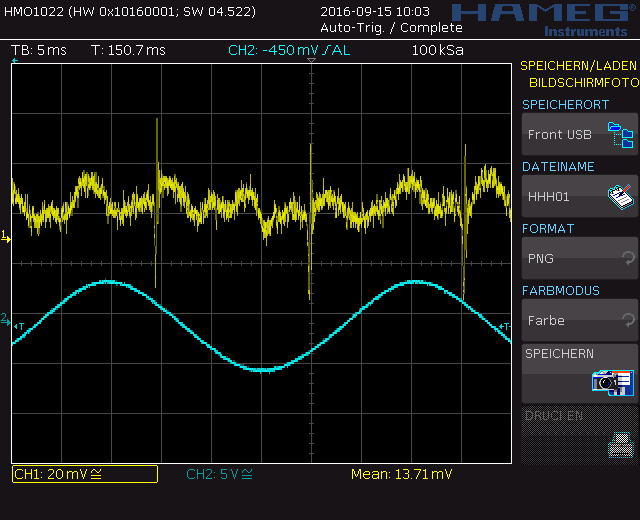
\includegraphics[width=0.4\textwidth]{data/HHH01.PNG}\hskip 10 pt
	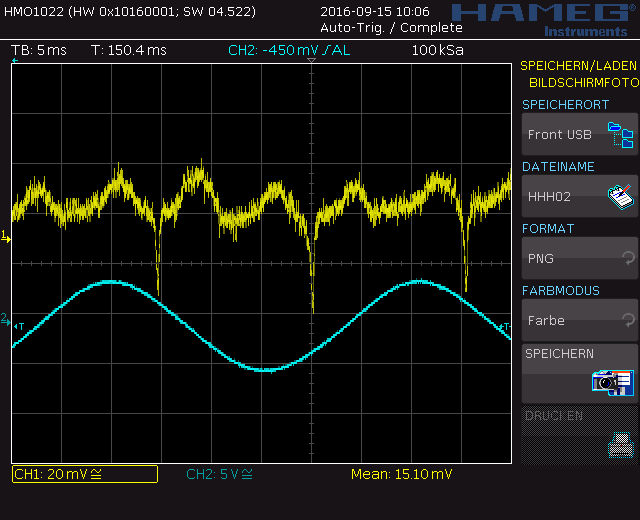
\includegraphics[width=0.4\textwidth]{data/HHH02.PNG}\vskip 10 pt
	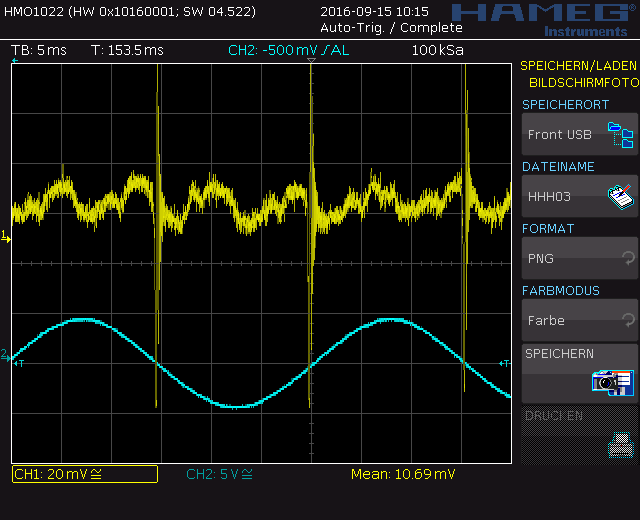
\includegraphics[width=0.4\textwidth]{data/HHH03.PNG}\hskip 10 pt
	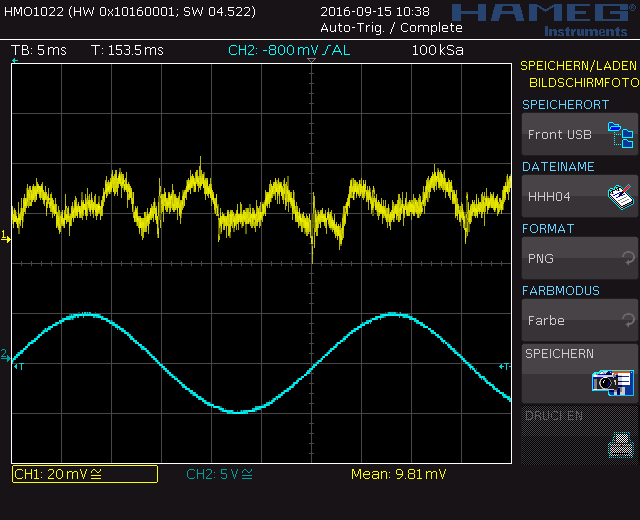
\includegraphics[width=0.4\textwidth]{data/HHH04.PNG}
	\captionof{figure}{Bilder der Resonanzfrequenzen von a) Proton im Wasserstoff, b) Proton in Glykol, c) Fluor, d) Fluor in Teflon}
\end{minipage}
\vskip 30 pt

\subsection{Messmethode 2} \label{FUCKTHISSHIT}

\begin{minipage}[h!]{\textwidth}
	\centering
	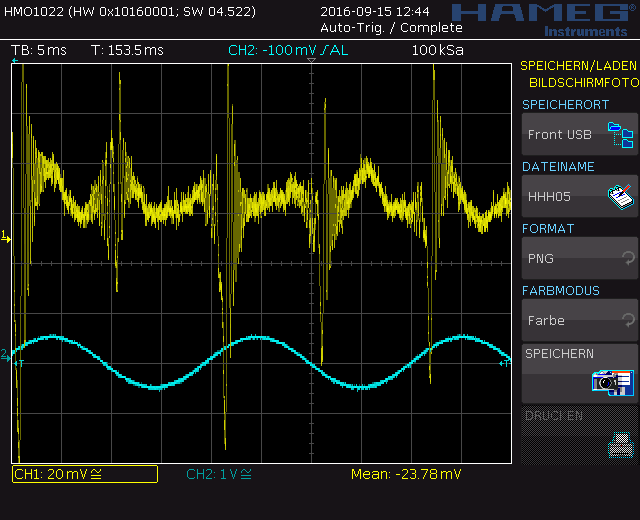
\includegraphics[width=0.4\textwidth]{data/HHH05.PNG}\hskip 10 pt
	\captionof{figure}{Grobeinstellung der Resonanzfrequenz vom Proton im Wasserstoff}
\end{minipage}
\vskip 30 pt

\begin{minipage}[h!]{\textwidth}
	\centering
	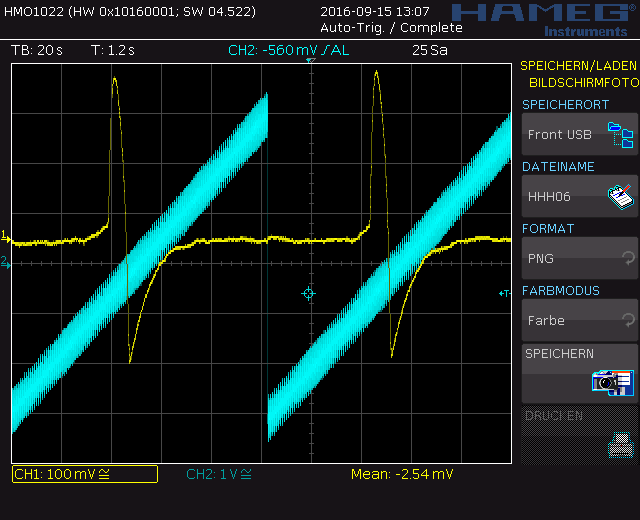
\includegraphics[width=0.4\textwidth]{data/HHH06.PNG}\hskip 10 pt
	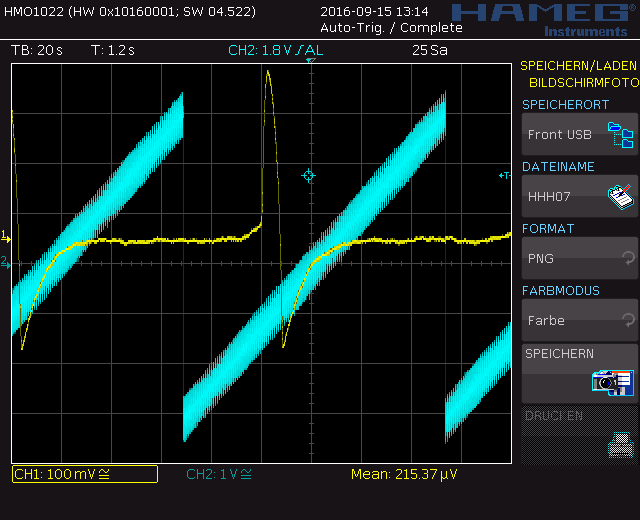
\includegraphics[width=0.4\textwidth]{data/HHH07.PNG}\vskip 10 pt
	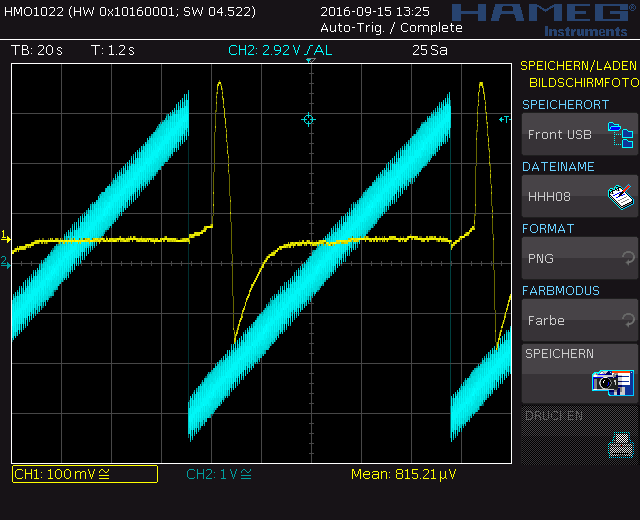
\includegraphics[width=0.4\textwidth]{data/HHH08.PNG}\hskip 10 pt
	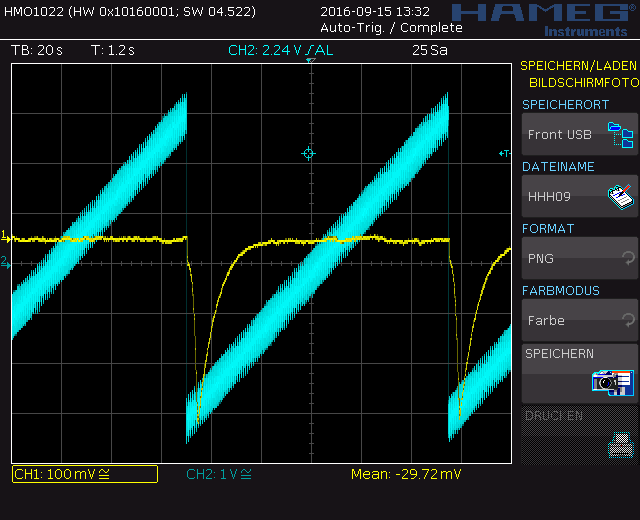
\includegraphics[width=0.4\textwidth]{data/HHH09.PNG}\vskip 10 pt
	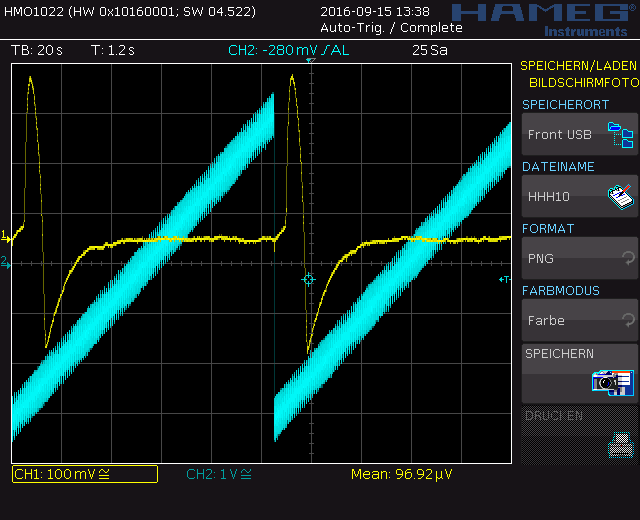
\includegraphics[width=0.4\textwidth]{data/HHH10.PNG}\hskip 10 pt
	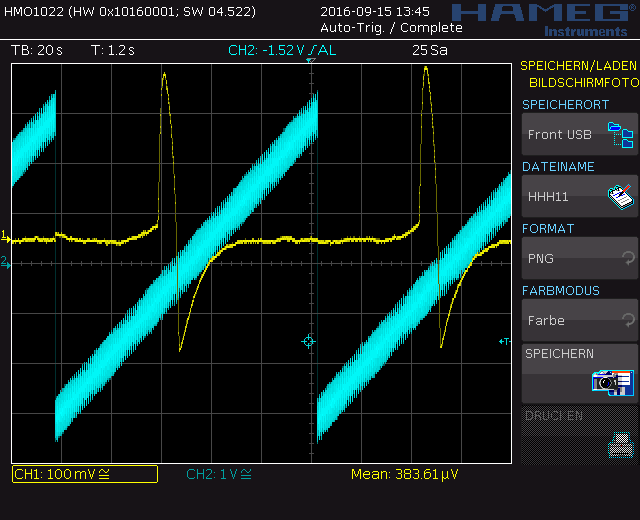
\includegraphics[width=0.4\textwidth]{data/HHH11.PNG}\vskip 10 pt
	\captionof{figure}{Bilder der differenzierten Absorptionskurven über dem Sägezahnsignal}
\end{minipage}
\begin{minipage}[h!]{\textwidth}
	\centering
	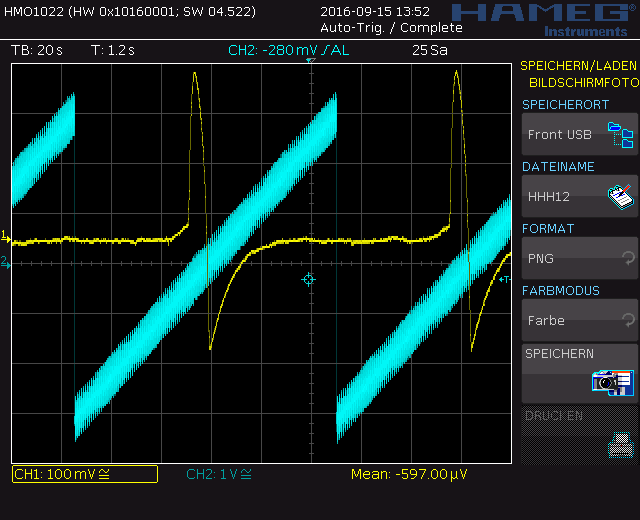
\includegraphics[width=0.4\textwidth]{data/HHH12.PNG}\hskip 10 pt
	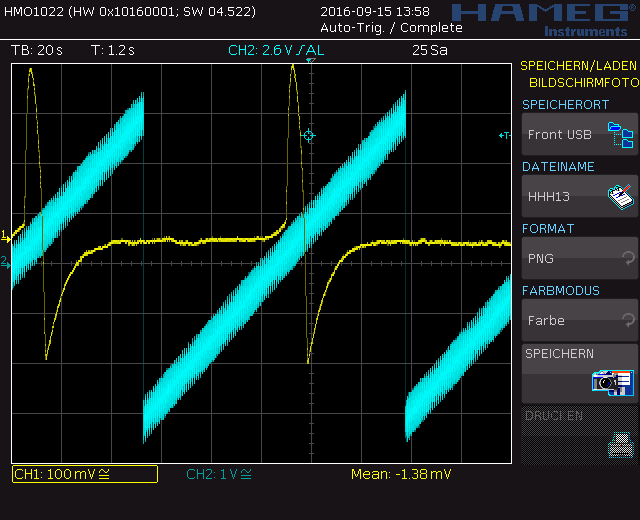
\includegraphics[width=0.4\textwidth]{data/HHH13.PNG}\vskip 10 pt	
	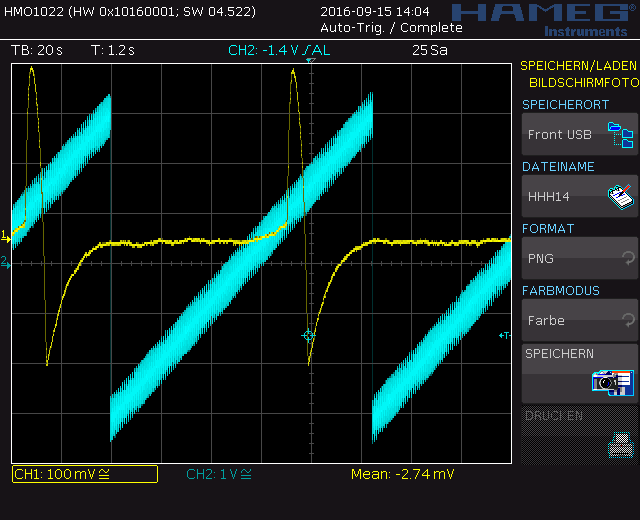
\includegraphics[width=0.4\textwidth]{data/HHH14.PNG}\hskip 10 pt
	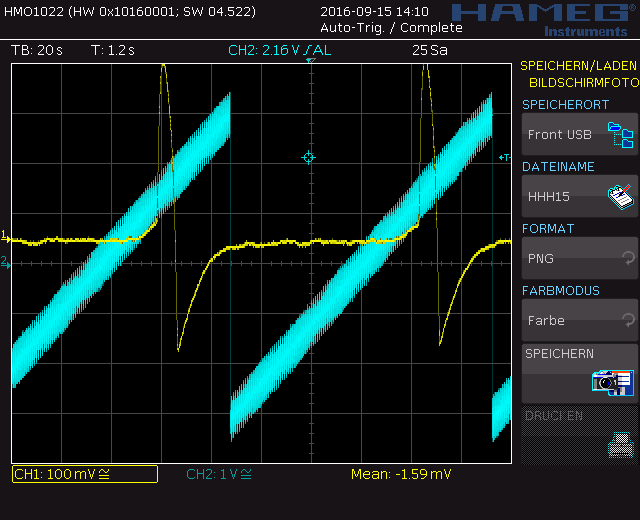
\includegraphics[width=0.4\textwidth]{data/HHH15.PNG}\vskip 10 pt
	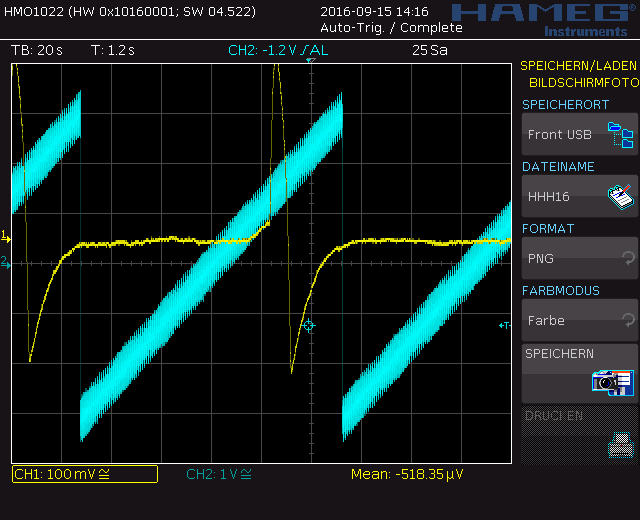
\includegraphics[width=0.4\textwidth]{data/HHH16.PNG}\hskip 10 pt
	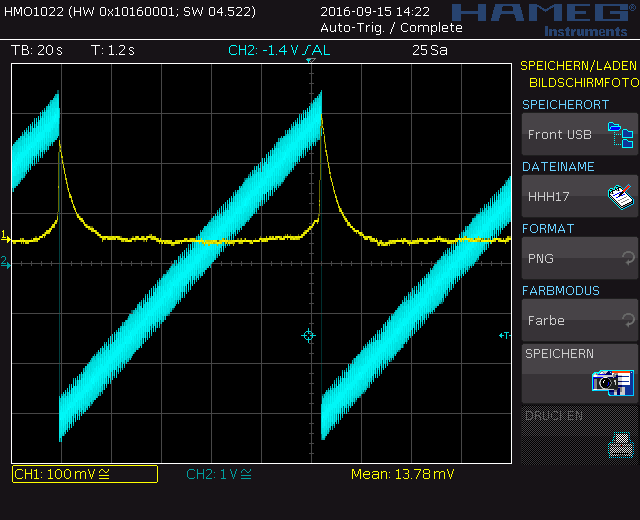
\includegraphics[width=0.4\textwidth]{data/HHH17.PNG}\vskip 10 pt
	\captionof{figure}{Bilder der differenzierten Absorptionskurven über dem Sägezahnsignal}
\end{minipage}

%\subsection{Tabellen}

%\subsubsection{$\alpha$-Plateau Samarium}
%\lstinputlisting[language=MATLAB]{Rohdaten/alphaPlateau_Sm.txt}


%\newpage
%\subsection{Quellcode (MATLAB)}
%\lstinputlisting[language=MATLAB]{Rohdaten/alpha.m}

\newpage
\subsection{Laborheft}
%\begin{minipage}{\textwidth}
%\centering
%\includegraphics[width=0.9\textwidth]{figures/IMG_20151002_141014.jpg}
%\end{minipage}

\newpage
\listoffigures

%Literatur----------------------------------------------------------------------------------------------------------

%\cite{les}
\newpage
\thispagestyle{empty}
\begin{thebibliography}{9}

%\bibitem{staat}
%  Tobijas Kotyk,
%  \emph{Versuche zur Radioaktivität im Physikalischen Fortgeschrittenen Praktikum an der Albert-Ludwigs-Universität Freiburg},
%  Albert-Ludwigs-Universität, Freiburg,
%  2005
  

  
%\bibitem{molmasse}
%  \emph{http://www.convertunits.com/molarmass/<ELEMENTNAME AUF ENGLISCH>}, Stand 28.09.2015
  
\bibitem{bibhall}
\emph{http://www.schule-bw.de/unterricht/faecher/physik/online\_material/e\_lehre\_2/teilchenfeld/\\halleffekt.htm}, Stand 15.09.2016

\bibitem{anleitung}
\emph{http://hacol13.physik.uni-freiburg.de/fp/Versuche/FP1/FP1-8-Kernspinresonanz/Anleitung.pdf}, Stand 15.09.2016

\bibitem{Babykatze}
\emph{http://hacol13.physik.uni-freiburg.de/fp/Versuche/FP1/FP1-8-Kernspinresonanz/Anhang/A.Klett.pdf}, Stand 19.09.2016
\end{thebibliography}

\end{document}